\section{Results}
\label{sec:results}

\subsection{Lever 1: Sharing Adds No Users}

One StreamSplat user alone, with the authors' \texttt{torch.compile}, takes 0.190~s per update and reaches 5.20 updates/s back to back. % log: G5
Its process holds 4,094~MiB, so memory alone would admit about 12 users. % log: G6
In all four settings of Table~\ref{tab:sharing}, time-slicing and MPS served the same number of users. % log: G2, G3, G6, G7
Every failing point failed on latency, never on memory. % log: G2, G6
Past capacity the GPU finished about the same number of updates per second under either mechanism. % log: G2, G6
At one keyframe per second, StreamSplat's rate was 4.62--4.73 updates/s, 9--11\% below one user alone. % log: G5, G6
Up to capacity, MPS lowered a user's latency measurably only at five AnySplat users with $k=2$. % log: G3

\begin{table}[t]
\centering
\footnotesize
\setlength{\tabcolsep}{3.5pt}
\begin{tabular}{@{}llcccc@{}}
\toprule
 & & \multicolumn{2}{c}{Users served} & \multicolumn{2}{c}{Saturated updates/s} \\
\cmidrule(lr){3-4}\cmidrule(l){5-6}
Model & Rate & TS & MPS & TS & MPS \\
\midrule
AnySplat, $k=8$ & 1/s & 2 & 2 & 2.52--2.53 & 2.45--2.47 \\ % log: G2
AnySplat, $k=2$ & 2/s & 5 & 5 & 10.07--10.09 & 10.18--10.29 \\ % log: G3
StreamSplat & 1/s & 4 & 4 & 4.71--4.73 & 4.62--4.65 \\ % log: G6
StreamSplat & 3/s & 1 & 1 & 4.77--4.83 & 4.81--4.95 \\ % log: G7
\midrule
\multicolumn{2}{@{}l}{Batch size $b$} & 1 & 2 & 4 & 8 \\
\multicolumn{2}{@{}l}{Updates/s, back to back} & 4.92 & 4.83 & 4.70 & 4.52 \\ % log: G9
\bottomrule
\end{tabular}
\caption{Top: users served with one process per user under time-slicing (TS) and MPS, and the throughput past capacity. % log: G2, G3, G6, G7
Rate is updates per user per second.
Bottom: the batching server, one run per batch size, on the released code. % log: G9
}
\label{tab:sharing}
\end{table}

Batching did not raise throughput either (Table~\ref{tab:sharing}, bottom).
A batch of 8 took 8.7 times as long as one update. % log: G9
GPU utilization rose from 72\% to 96\% while throughput fell, so the idle time at batch 1 was not capacity that batching could use. % log: G9
We had set 1.2 times the batch-1 throughput as the condition for a capacity sweep of the batching server, so we did not sweep it. % log: G9
With the bf16 model, batch 4 gave 0.96--1.04 times the batch-1 throughput. % log: G12, G13, G14
These results hold for the released code.
We did not combine time-slicing or MPS with Lever 2, and we measured batching after Lever 2 only back to back.

\subsection{Lever 2: Less Work per Update}

A profile of one update showed where to cut. % log: G10
The released code re-encodes the previous keyframe at every update, 21.5\% of the forward pass. % log: G10
In FP32, PyTorch's attention has no FlashAttention kernel, and attention takes 67\% of kernel time. % log: G10
Under bf16, attention takes 25\% of kernel time, and the forward pass runs 2.4 times faster. % log: G10

\begin{table}[t]
\centering
\footnotesize
\setlength{\tabcolsep}{2.5pt}
\begin{tabular}{@{}lccccc@{}}
\toprule
 & Updates/s & \multicolumn{2}{c}{Speedup} & Memory & Keyframe \\
\cmidrule(lr){3-4}
Optimization & $b=1$ & $b=1$ & $b=4$ & (MiB) & PSNR (dB) \\
\midrule
Feature cache & 4.68$\to$5.93 & 1.27 & 1.21 & $+0$ & --$^{a}$ \\ % log: G11
bf16 model & 6.13$\to$10.83 & 1.77 & 1.95 & $+16$ & $-0.18$ \\ % log: G12
No host sync & 11.00$\to$10.73 & 0.98 & 1.01 & $+0$ & --$^{b}$ \\ % log: G13
CUDA graphs & 10.97$\to$11.54 & 1.05 & 0.99 & $+162$ to $+460$ & --$^{b}$ \\ % log: G14
bf16 depth & 11.64$\to$15.71 & 1.35 & -- & $-162$ to $-52^{c}$ & $-0.013$ \\ % log: G16
\bottomrule
\end{tabular}
\caption{Each optimization against its matched control, interleaved, 2 repeats per cell. % log: G11-G14, G16
Each control has every optimization above it, and the graphs control also has checkpointing off.
Updates/s is the mean back-to-back throughput from control to treatment.
Memory is the change in whole-GPU memory at $b=1$.
Keyframe PSNR is the mean change on DAVIS 2017 val against the previous step.
$^{a}$Not evaluated on DAVIS. Mean absolute difference from the control's Gaussians: $4.2\times10^{-8}$ in FP32. % log: G11
$^{b}$Not evaluated on DAVIS. Output bitwise identical to the control's. % log: G13, G14
$^{c}$At 10 to 12 users in the capacity sweep.} % log: G16
\label{tab:ablation}
\end{table}

Table~\ref{tab:ablation} gives each optimization against a control that lacks only it.
The cache and the bf16 model gave the largest gains, 1.27 and 1.77 times. % log: G11, G12
Removing the host synchronizations gave 0.98 times, and we kept it because CUDA graphs need it. % log: G13
CUDA graphs gave 1.05 times, so kernel launches cost little. % log: G14
The ratios depend on the order and do not multiply into a total.
Measured directly, \opt{} runs 11.53 updates/s back to back, 2.33 times \serial{}'s 4.95. % log: G15

\begin{figure}[t]
\centering
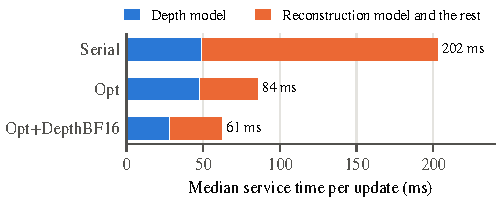
\includegraphics[width=\columnwidth]{figures/breakdown}
\caption{Median service time per update, back to back at $b=1$, split into the depth stage (upload included) and the rest. % log: G15, G16
\serial{} is one run, and \opt{} and \optd{} are means of 2 runs.} % log: G15, G16
\label{fig:breakdown}
\end{figure}

After these steps, the depth stage took 47.1 of \opt{}'s 84.2~ms per update (Figure~\ref{fig:breakdown}). % log: G16
Running it under bf16 cut the depth stage to 27.5~ms and raised throughput 1.35 times. % log: G16
The depth stage is still 45\% of an \optd{} update. % log: G16

\subsection{Goals 1 and 2: More Users, Lower Latency}

\begin{table}[t]
\centering
\footnotesize
\setlength{\tabcolsep}{3pt}
\begin{tabular}{@{}lrrrrr@{}}
\toprule
 & Back to back & Capacity & p95 at & \multicolumn{2}{c}{Memory (MiB)} \\
\cmidrule(l){5-6}
Configuration & (updates/s) & (users) & capacity (s) & total & per user \\
\midrule
\serial{} & 4.95 & 4 & 0.205--0.209 & 3,892 & 973 \\ % log: G15
\opt{} & 11.53--11.64 & 10 & 0.094--0.100 & 4,928 & 493 \\ % log: G15, G16
\optd{} & 15.71 & 14 & 0.074--0.087 & 4,884 & 349 \\ % log: G16
\bottomrule
\end{tabular}
\caption{Capacity at one keyframe per user per second.
p95 is the worst user's in each repeat at capacity, and memory is the whole GPU's maximum at capacity. % log: G15, G16
\opt{} ran in two sweeps, and its ranges cover both.}
\label{tab:capacity}
\end{table}

Table~\ref{tab:capacity} gives the capacity of each configuration: 4 users for \serial{}, 10 for \opt{} and 14 for \optd{}. % log: G15, G16
\opt{} failed both repeats at 11 users, and \optd{} passed 15 users in one repeat of two. % log: G16
Below capacity, the worst p95 stays close to one update's service time (Figure~\ref{fig:latency}). % log: G15, G16
At 4 users it is 0.207~s for \serial{} and 0.090~s for \opt{}. % log: G15
At 10 users it is 0.097~s for \opt{} and 0.076~s for \optd{}. % log: G16
Where neither repeat passed, the queue grew for the whole run, and the worst p95 reached 2.3--12.0~s. % log: G15, G16

\begin{figure}[t]
\centering
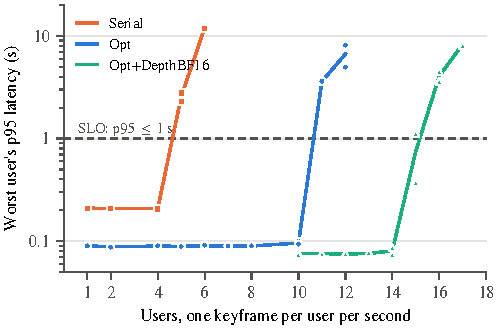
\includegraphics[width=\columnwidth]{figures/latency}
\caption{Worst user's p95 latency against the number of users, each sending one keyframe per second, on a log scale. % log: G15, G16
Markers are single repeats, and lines join the means.
\opt{} combines its two sweeps, so it has four markers at 10 and 12 users.
The dashed line is the 1~s SLO.} % log: G15, G16
\label{fig:latency}
\end{figure}

Capacity stops short of the back-to-back throughput.
The SLO held up to about 0.89 of that rate and failed from about 0.95 of it. % log: G16
Past capacity, \opt{}'s median service time also grew, from 84.2~ms back to back to 96.3--96.7~ms. % log: G16
Memory stayed far from the limit: at capacity the card held at most 4,928~MiB, about 10\% of it. % log: G15, G16
All users share one process and one copy of the weights.
In both optimized configurations, each added user costs about 25~MiB of live tensors. % log: G15, G16

\subsection{Goal 3: Keeping the Quality}

\begin{table}[t]
\centering
\footnotesize
\setlength{\tabcolsep}{3.5pt}
\begin{tabular}{@{}lrrrr@{}}
\toprule
 & \multicolumn{2}{c}{PSNR (dB)} & \multicolumn{2}{c}{Keyframes vs.\ full} \\
\cmidrule(lr){2-3}\cmidrule(l){4-5}
Precision & keyframes & middle & mean (dB) & $>$0.5~dB loss \\
\midrule
Paper~\cite{streamsplat2026} & 37.83 & 23.66 & & \\ % log: G8
Full precision & 37.76 & 23.76 & -- & -- \\ % log: G8
bf16 model & 37.58 & 23.75 & $-0.18$ & 4.3\% \\ % log: G12
bf16 model and depth & 37.57 & 23.75 & $-0.19$ & 5.1\% \\ % log: G16
\bottomrule
\end{tabular}
\caption{Quality on the 1,849 DAVIS 2017 validation windows with the authors' metric. % log: G8
The last two columns pair each window with its full-precision result.}
\label{tab:quality}
\end{table}

Table~\ref{tab:quality} gives the quality cost.
The bf16 model lowered keyframe PSNR by 0.18~dB, and the bf16 depth model by a further 0.013~dB. % log: G12, G16
The total loss is 0.19~dB on keyframes and 0.01~dB on middle frames. % log: G16
5.1\% of the windows lose more than 0.5~dB of keyframe PSNR. % log: G16
A rerun on two sequences reproduced all 64 of their windows bitwise, so these differences carry no run-to-run noise. % log: G16
The evaluation runs the model's uncached forward pass with keyframes five frames apart. % log: G8, G16
The server uses keyframes one second apart, and we did not measure quality at that spacing.
